
\let\negmedspace\undefined
\let\negthickspace\undefined
\documentclass[journal,12pt,twocolumn]{IEEEtran}
%\documentclass[conference]{IEEEtran}
%\IEEEoverridecommandlockouts
% The preceding line is only needed to identify funding in the first footnote. If that is unneeded, please comment it out.
\usepackage{cite}
\usepackage{amsmath,amssymb,amsfonts,amsthm}
\usepackage{algorithmic}
\usepackage{graphicx}
\usepackage{textcomp}
\usepackage{xcolor}
\usepackage{txfonts}
\usepackage{listings}
\usepackage{enumitem}
\usepackage{mathtools}
\usepackage{gensymb}
\usepackage[breaklinks=true]{hyperref}
\usepackage{tkz-euclide} % loads  TikZ and tkz-base
\usepackage{listings}
%
%\usepackage{setspace}
%\usepackage{gensymb}
%\doublespacing
%\singlespacing

%\usepackage{graphicx}
%\usepackage{amssymb}
%\usepackage{relsize}
%\usepackage[cmex10]{amsmath}
%\usepackage{amsthm}
%\interdisplaylinepenalty=2500
%\savesymbol{iint}
%\usepackage{txfonts}
%\restoresymbol{TXF}{iint}
%\usepackage{wasysym}
%\usepackage{amsthm}
%\usepackage{iithtlc}
%\usepackage{mathrsfs}
%\usepackage{txfonts}
%\usepackage{stfloats}
%\usepackage{bm}
%\usepackage{cite}
%\usepackage{cases}
%\usepackage{subfig}
%\usepackage{xtab}
%\usepackage{longtable}
%\usepackage{multirow}
%\usepackage{algorithm}
%\usepackage{algpseudocode}
%\usepackage{enumitem}
%\usepackage{mathtools}
%\usepackage{tikz}
%\usepackage{circuitikz}
%\usepackage{verbatim}
%\usepackage{tfrupee}
%\usepackage{stmaryrd}
%\usetkzobj{all}
%    \usepackage{color}                                            %%
%    \usepackage{array}                                            %%
%    \usepackage{longtable}                                        %%
%    \usepackage{calc}                                             %%
%    \usepackage{multirow}                                         %%
%    \usepackage{hhline}                                           %%
%    \usepackage{ifthen}                                           %%
  %optionally (for landscape tables embedded in another document): %%
%    \usepackage{lscape}     
%\usepackage{multicol}
%\usepackage{chngcntr}
%\usepackage{enumerate}

\providecommand{\mbf}{\mathbf}
\providecommand{\pr}[1]{\ensuremath{\Pr\left(#1\right)}}
\providecommand{\qfunc}[1]{\ensuremath{Q\left(#1\right)}}
\providecommand{\sbrak}[1]{\ensuremath{{}\left[#1\right]}}
\providecommand{\lsbrak}[1]{\ensuremath{{}\left[#1\right.}}
\providecommand{\rsbrak}[1]{\ensuremath{{}\left.#1\right]}}
\providecommand{\brak}[1]{\ensuremath{\left(#1\right)}}
\providecommand{\lbrak}[1]{\ensuremath{\left(#1\right.}}
\providecommand{\rbrak}[1]{\ensuremath{\left.#1\right)}}
\providecommand{\cbrak}[1]{\ensuremath{\left\{#1\right\}}}
\providecommand{\lcbrak}[1]{\ensuremath{\left\{#1\right.}}
\providecommand{\rcbrak}[1]{\ensuremath{\left.#1\right\}}}
\theoremstyle{remark}
\newtheorem{rem}{Remark}
\newcommand{\sgn}{\mathop{\mathrm{sgn}}}
%\providecommand{\abs}[1]{\left\vert#1\right\vert}
\providecommand{\res}[1]{\Res\displaylimits_{#1}} 
%\providecommand{\norm}[1]{\left\lVert#1\right\rVert}
%\providecommand{\norm}[1]{\lVert#1\rVert}
\providecommand{\mtx}[1]{\mathbf{#1}}
\providecommand{\mean}[1]{E\left[ #1 \right]}
\providecommand{\fourier}{\overset{\mathcal{F}}{ \rightleftharpoons}}
%\providecommand{\hilbert}{\overset{\mathcal{H}}{ \rightleftharpoons}}
\providecommand{\system}{\overset{\mathcal{H}}{ \longleftrightarrow}}
	%\newcommand{\solution}[2]{\textbf{Solution:}{#1}}
\newcommand{\solution}{\noindent \textbf{Solution: }}
\newcommand{\cosec}{\,\text{cosec}\,}
\providecommand{\dec}[2]{\ensuremath{\overset{#1}{\underset{#2}{\gtrless}}}}
\newcommand{\myvec}[1]{\ensuremath{\begin{pmatrix}#1\end{pmatrix}}}
\newcommand{\mydet}[1]{\ensuremath{\begin{vmatrix}#1\end{vmatrix}}}
%\usepackage{wasysym}
%\newcounter{MYtempeqncnt}
\DeclareMathOperator*{\Res}{Res}
%\renewcommand{\baselinestretch}{2}
\renewcommand\thesection{\arabic{section}}
\renewcommand\thesubsection{\thesection.\arabic{subsection}}
\renewcommand\thesubsubsection{\thesubsection.\arabic{subsubsection}}

\renewcommand\thesectiondis{\arabic{section}}
\renewcommand\thesubsectiondis{\thesectiondis.\arabic{subsection}}
\renewcommand\thesubsubsectiondis{\thesubsectiondis.\arabic{subsubsection}}
%new commands 
\newcommand{\permcomb}[4][0mu]{{{}^{#3}\mkern#1#2_{#4}}}
\newcommand{\comb}[1][-1mu]{\permcomb[#1]{C}}

% correct bad hyphenation here
\hyphenation{op-tical net-works semi-conduc-tor}
\def\inputGnumericTable{}                                 %%

\lstset{
%language=C,
frame=single, 
breaklines=true,
columns=fullflexible
}
%\lstset{
%language=tex,
%frame=single, 
%breaklines=true
%}

\title{

  Assignment:- 2\\
  \Large AI1110: Probability and Random Variables\\
  \Large Indian Institute of Technology, Hyderabad
}
\author{
  CS22BTECH11017\\[4pt]
  Dikshant Khandelwal\\
  11th May, 2023
  % <-this % stops a space
}
\begin{document}
%

\maketitle

\textbf{Exercise 12.13.1.10} A black and a red dice are rolled.
\begin{enumerate}[label=(\alph*)]
    \item Find the conditional probability of obtaining a sum greater than 9, given
that the black die resulted in a 5.
    \item Find the conditional probability of obtaining the sum 8, given that the red die
resulted in a number less than 4.
\end{enumerate}

\textbf{Solution.} Let $X$ and $Y$ be the random variables denoting the number which comes up on black and red die respectively.\\
Let us define cumulative frequency distribution of some random variable A,
\begin{align}
    F_{A}(i) &= \pr{A \le i}\\
    \therefore  \label{cdf}F_{X}(i) = F_{Y}(i) &= 
              \begin{cases} 0  & i<1\\
                            \frac{i}{6} & 0 < i \le 6\\
                            1 & i> 6
              \end{cases}
\end{align}
$X$ and $Y$ are independent random variables.
\begin{align}
    \pr{X =k , Y =r} &= \pr{X = k} \pr{Y= r}\\
    \therefore \pr{X =k , Y =r} &= \frac{1}{36}
\end{align}

\begin{enumerate}[label=(\alph*)]
    \item
    \begin{align}
        \pr{X+Y> 9 | X = 5} &= \frac{\pr{X+Y> 9, X = 5}}{\pr{X = 5}}\\
                          &= \pr{Y > 4}\\
                          &= F_{Y}(6) -F_{Y}(4)\\
                          &= 1 - \frac{4}{6}\\
                          &= \frac{1}{3} \approx 0.33\\
                          \therefore \pr{X+Y> 9 | X = 5} &= \frac{1}{3}\approx 0.33
    \end{align}
\item

\begin{align}
\pr{X+Y = 8 | Y < 4} &= \frac{\pr{X+Y = 8, Y < 4}}{\pr{Y < 4}}
\end{align}

\begin{figure}[h!]
  \centering 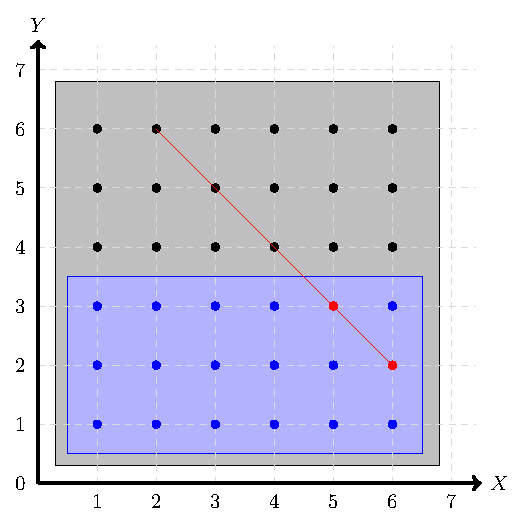
\includegraphics[width= 7.15cm]{figs/figure}
  \caption{$X+Y = 8 | Y < 4$}
  \label{fig:1}
\end{figure}



Probability of an event $E$, written as $\pr{E}$
\begin{align}
\pr{E}=\frac{\text{Number of outcomes favourable to $E$}}{\text{Total Number of possible outcomes }}
\end{align}

\begin{align}
    \pr{Y < 4} &= \frac{\text{Number of $(X,Y)$ in blue region}}{\text{Number of $(X,Y)$ in gray region }}\\
    &= \frac{\brak{3}\cdot\brak{6}}{\brak{6}\cdot\brak{6}}\\
    &= \frac{1}{2}
\end{align}

\begin{align}
    \pr{X+Y = 8, Y<4} &= \frac{\text{Number of red dots $(X,Y)$ }}{\text{Number of $(X,Y)$ in gray region }}\\
    &= \frac{2}{\brak{6}\cdot\brak{6}}\\
         &=\frac{1}{18} 
    \end{align}
    \begin{align}
    \therefore \pr{X+Y = 8 | Y < 4} &= \frac{\brak{\frac{1}{18}}}{\brak{\frac{1}{2}}}\\
    &=\frac{1}{9} \approx 0.11
\end{align}


\end{enumerate}

\end{document}


